\chapter{Sobre Tipografia}
\label{ch:Tipografia}

O ensino de tipografia a deficientes visuais requer a transformação das formas e dos conceitos visuais em modelos táteis. Neste capítulo, definem-se quais conceitos serão trabalhados, identificando as partes estruturais das letras, que apresentam distinções de acordo com a tipografia a qual pertencem. Neste capítulo são apresentados esses conceitos e detalhados os fundamentos deste projeto.

\section{Conceitos Gerais}

A tipografia é a comunicação escrita por meio de tipos \citeC{bierut2010}.Surgiu na Alemanha na década de 1450, quando aliaram-se os tipos móveis de metal à prensa, resultando no primeiro livro impresso \citeC{bringhurst2005}.  A diferença entre a letra escrita e a tipográfica são os método utilizados para gerar as letras \citeC{lupton2014}. Por exemplo, existem fontes de letra cursiva, que apesar da aparência de caligrafia, na realidade, são tipografia, uma vez que são geradas por uma definição de fonte de computador.  Sendo assim, para ser considerar-se tipografia, o processo deve ser regulado por máquina. Na era digital, os tipos móveis foram adaptados para o que chamamos de fontes, apesar de o termo ser usado erroneamente. Fonte diz respeito ao software e já tipo, à configuração visual \citeC{lupton2014}.

Dentro da tipografia, existem alguns parâmetros que determinam as configurações de um tipo. As linhas-guia, por exemplo, são linhas que determinam limites horizontais para as letras em dado tipo. Essas linhas-guia são classificadas como linha das ascendentes, linha mediana, linha de base e linha das ascendentes, que são ilustradas na Figura  \ref{fig:linhas}. A linha de base serve para o alinhamento de todas as letras. Já a linha mediana indica a altura-x, ou seja, a altura das letras minúsculas. A linha das ascendentes delimita as letras que se projetam acima da linha de base e a linha das descendentes, das que se projetam abaixo da linha de base \citeC{kane2012}.

\begin{figure}[H]
 \centering
  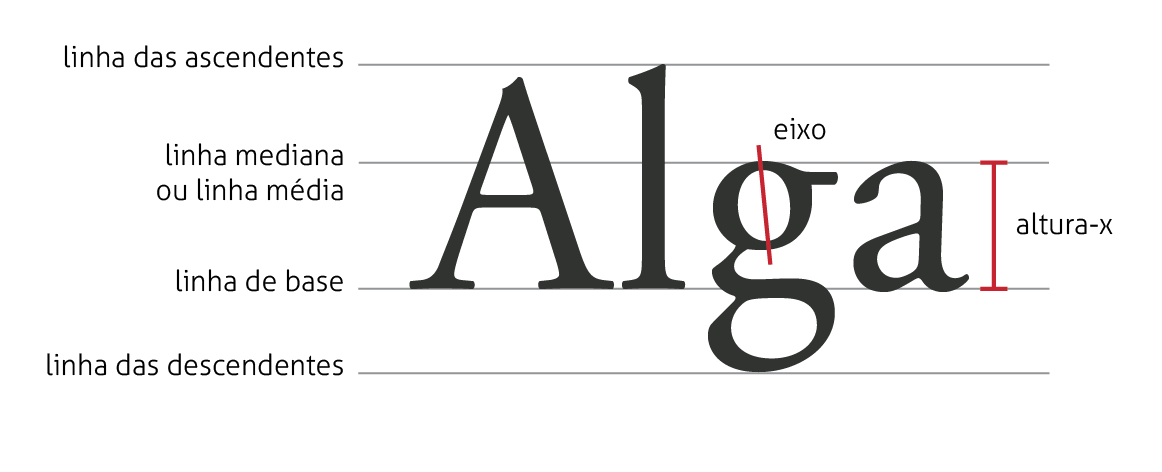
\includegraphics[width=0.75\linewidth]{figuras/linhas.pdf}
  \caption{Ilustração de mapeamento de conjunto de dados de treinamento em novo espaço de características a partir da utilização de função \textit{kernel}, possibilitando a divisão linear entre as categorias.}
  \label{fig:linhas}
\end{figure}


A relação entre a altura-x e altura das capitulares é o que vai fazer com que um tipo pareça maior ou menor em uma mesma quantidade de pontos. Quanto menor for a diferença entre essas duas alturas, maior será a aparência do tipo e maior a sua legibilidade, principalmente em tamanhos pequenos. A unidade de medida usualmente utilizada para a medição de tipos é o ponto, que é equivalente a 0,35 mm.  A contagem dos pontos em determinado tipo é feita desde a linha das ascendentes até a linha das descendentes \citeC{lupton2014}.

Outros parâmetros moldam a aparência de um tipo como o contraste, a inclinação, o eixo e a largura. O contraste é definido como a diferença entre traços finos e grossos. Já o eixo é o ângulo no qual se constroem as letras e, por último, a largura é a extensão horizontal das letras.

Outro conceito importante no campo da tipografia é chamado de anatomia da letra, que são termos técnicos para especificar determinada parte de uma letra, como está ilustrado na Figura \ref{fig:anatomia}.

\begin{figure}[H]
 \centering
  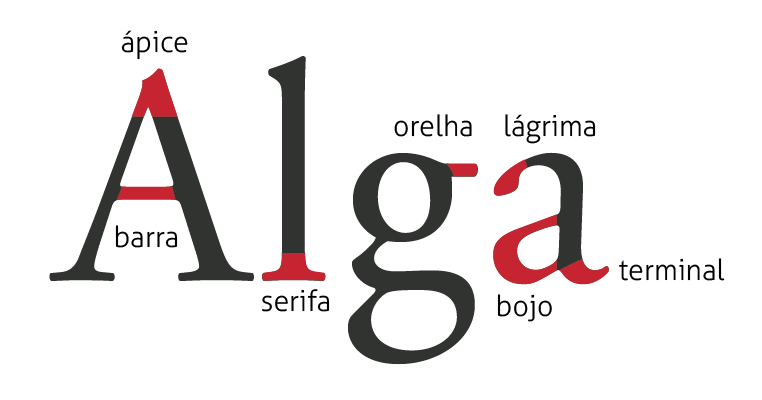
\includegraphics[width=0.45\linewidth]{figuras/anatomia.pdf}
  \caption{Ilustração de mapeamento de conjunto de dados de treinamento em novo espaço de características a partir da utilização de função \textit{kernel}, possibilitando a divisão linear entre as categorias.}
  \label{fig:anatomia}
\end{figure}

\section{Classificação Tipográfica}

As classificações tipográficas surgiram com a intenção de criar uniformidade na definição e descrição dos tipos. Ainda que não exista uma versão oficial na área da tipografia, a classificação criada por Maximilien Vox, adaptada posteriormente pela Associação Tipográfica Internacional (ATypi), é uma das classificações mais reconhecidas e utilizadas atualmente. Esta classificação,  conhecida como classificação Vox ATypi, une características históricas e estéticas e é dividida em grupos e subgrupos, conforme ilustrado na Figura \ref{fig:categoria} \citeC{rocha2012}.

\begin{figure}[H]
 \centering
  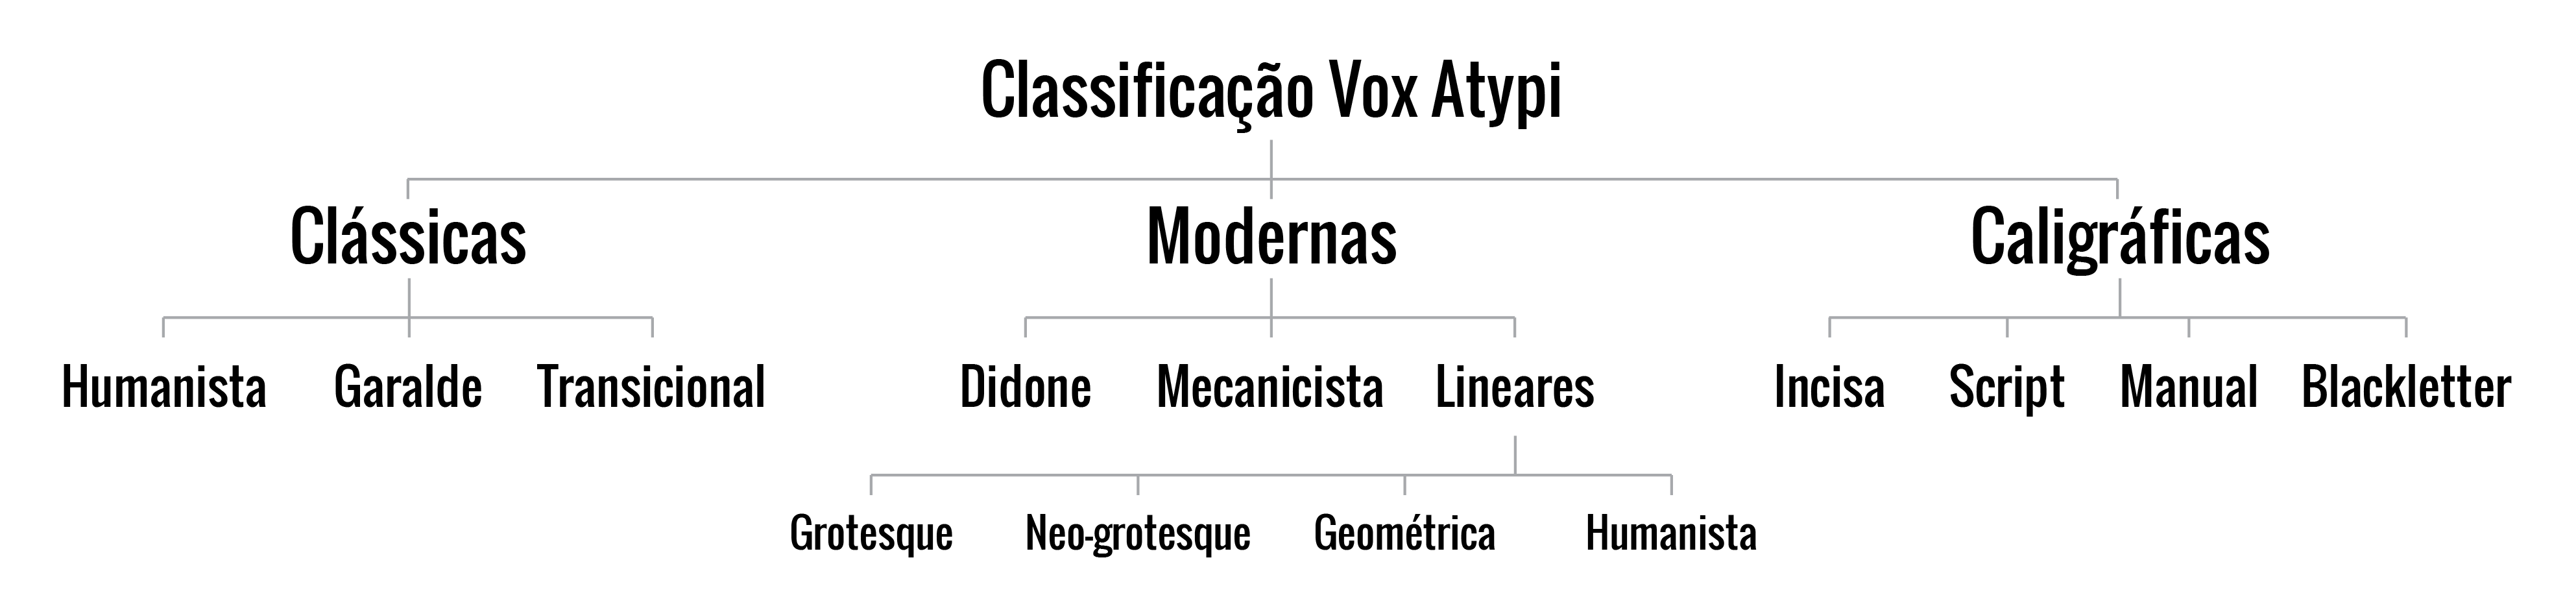
\includegraphics[width=1\linewidth]{figuras/classVox.pdf}
  \caption{Sistema de classificação tipográfica Vox ATpyi \citeC{cruz2017}}
  \label{fig:categoria}
\end{figure}

O sistema divide-se em três grupos principais de tipografia: clássicas, modernas e caligráficas. Cada grupo é também dividido em alguns subgrupos, que são listados a seguir \citeC{cruz2017}.

\begin{enumerate}
\item Caligráficas: incisa, \textit{script}, manual e \textit{blackletter};
\item Clássicas: humanista, \textit{garalde} e transicionais;
\item Modernas: \textit{didone} e mecanicista;
\item Lineares: \textit{grotesque}, \textit{neo-grotesques}, geométrica e humanista.
\end{enumerate}

Neste projeto, essa classificação é utilizada como modelo guia para a escolha das tipografias. A partir das categorias presentes na classificação citada, é possível definir uma estrutura que permite apresentar a tipografia por um panorâma histórico. Desta forma, é possível descrever como a tipografia evoluiu de acordo com as técnicas empregadas e com as correntes filosóficas contemporâneas, sendo esta uma abordagem interessante para o projeto.

Sendo assim, foi escolhida uma tipografia representante de cada categoria, excluindo-se a categoria caligráfica, por não pertencer ao escopo principal do projeto em primeiro momento, já que tem como intuito uma representação caligráfica e não tipográfica. As tipografias adotadas foram escolhidas devido à sua relevância histórica, estão listadas a seguir e são ilustradas na Figura \ref{fig:categoriasProjeto}.

\begin{enumerate}
\item Humanista: Adobe Jenson;
\item \textit{Garalde}: Adobe Garamond;
\item Transicional: Baskerville;
\item Didone: Didot;
\item Mecanicista: Clarendon;
\item Grotesque: Franklin Gothic URW;
\item Neo-grotesque: Helvetica;
\item Geométrica: Futura;
\item Humanista: Gill Sans.
\end{enumerate}

\begin{figure}[H]
 \centering
  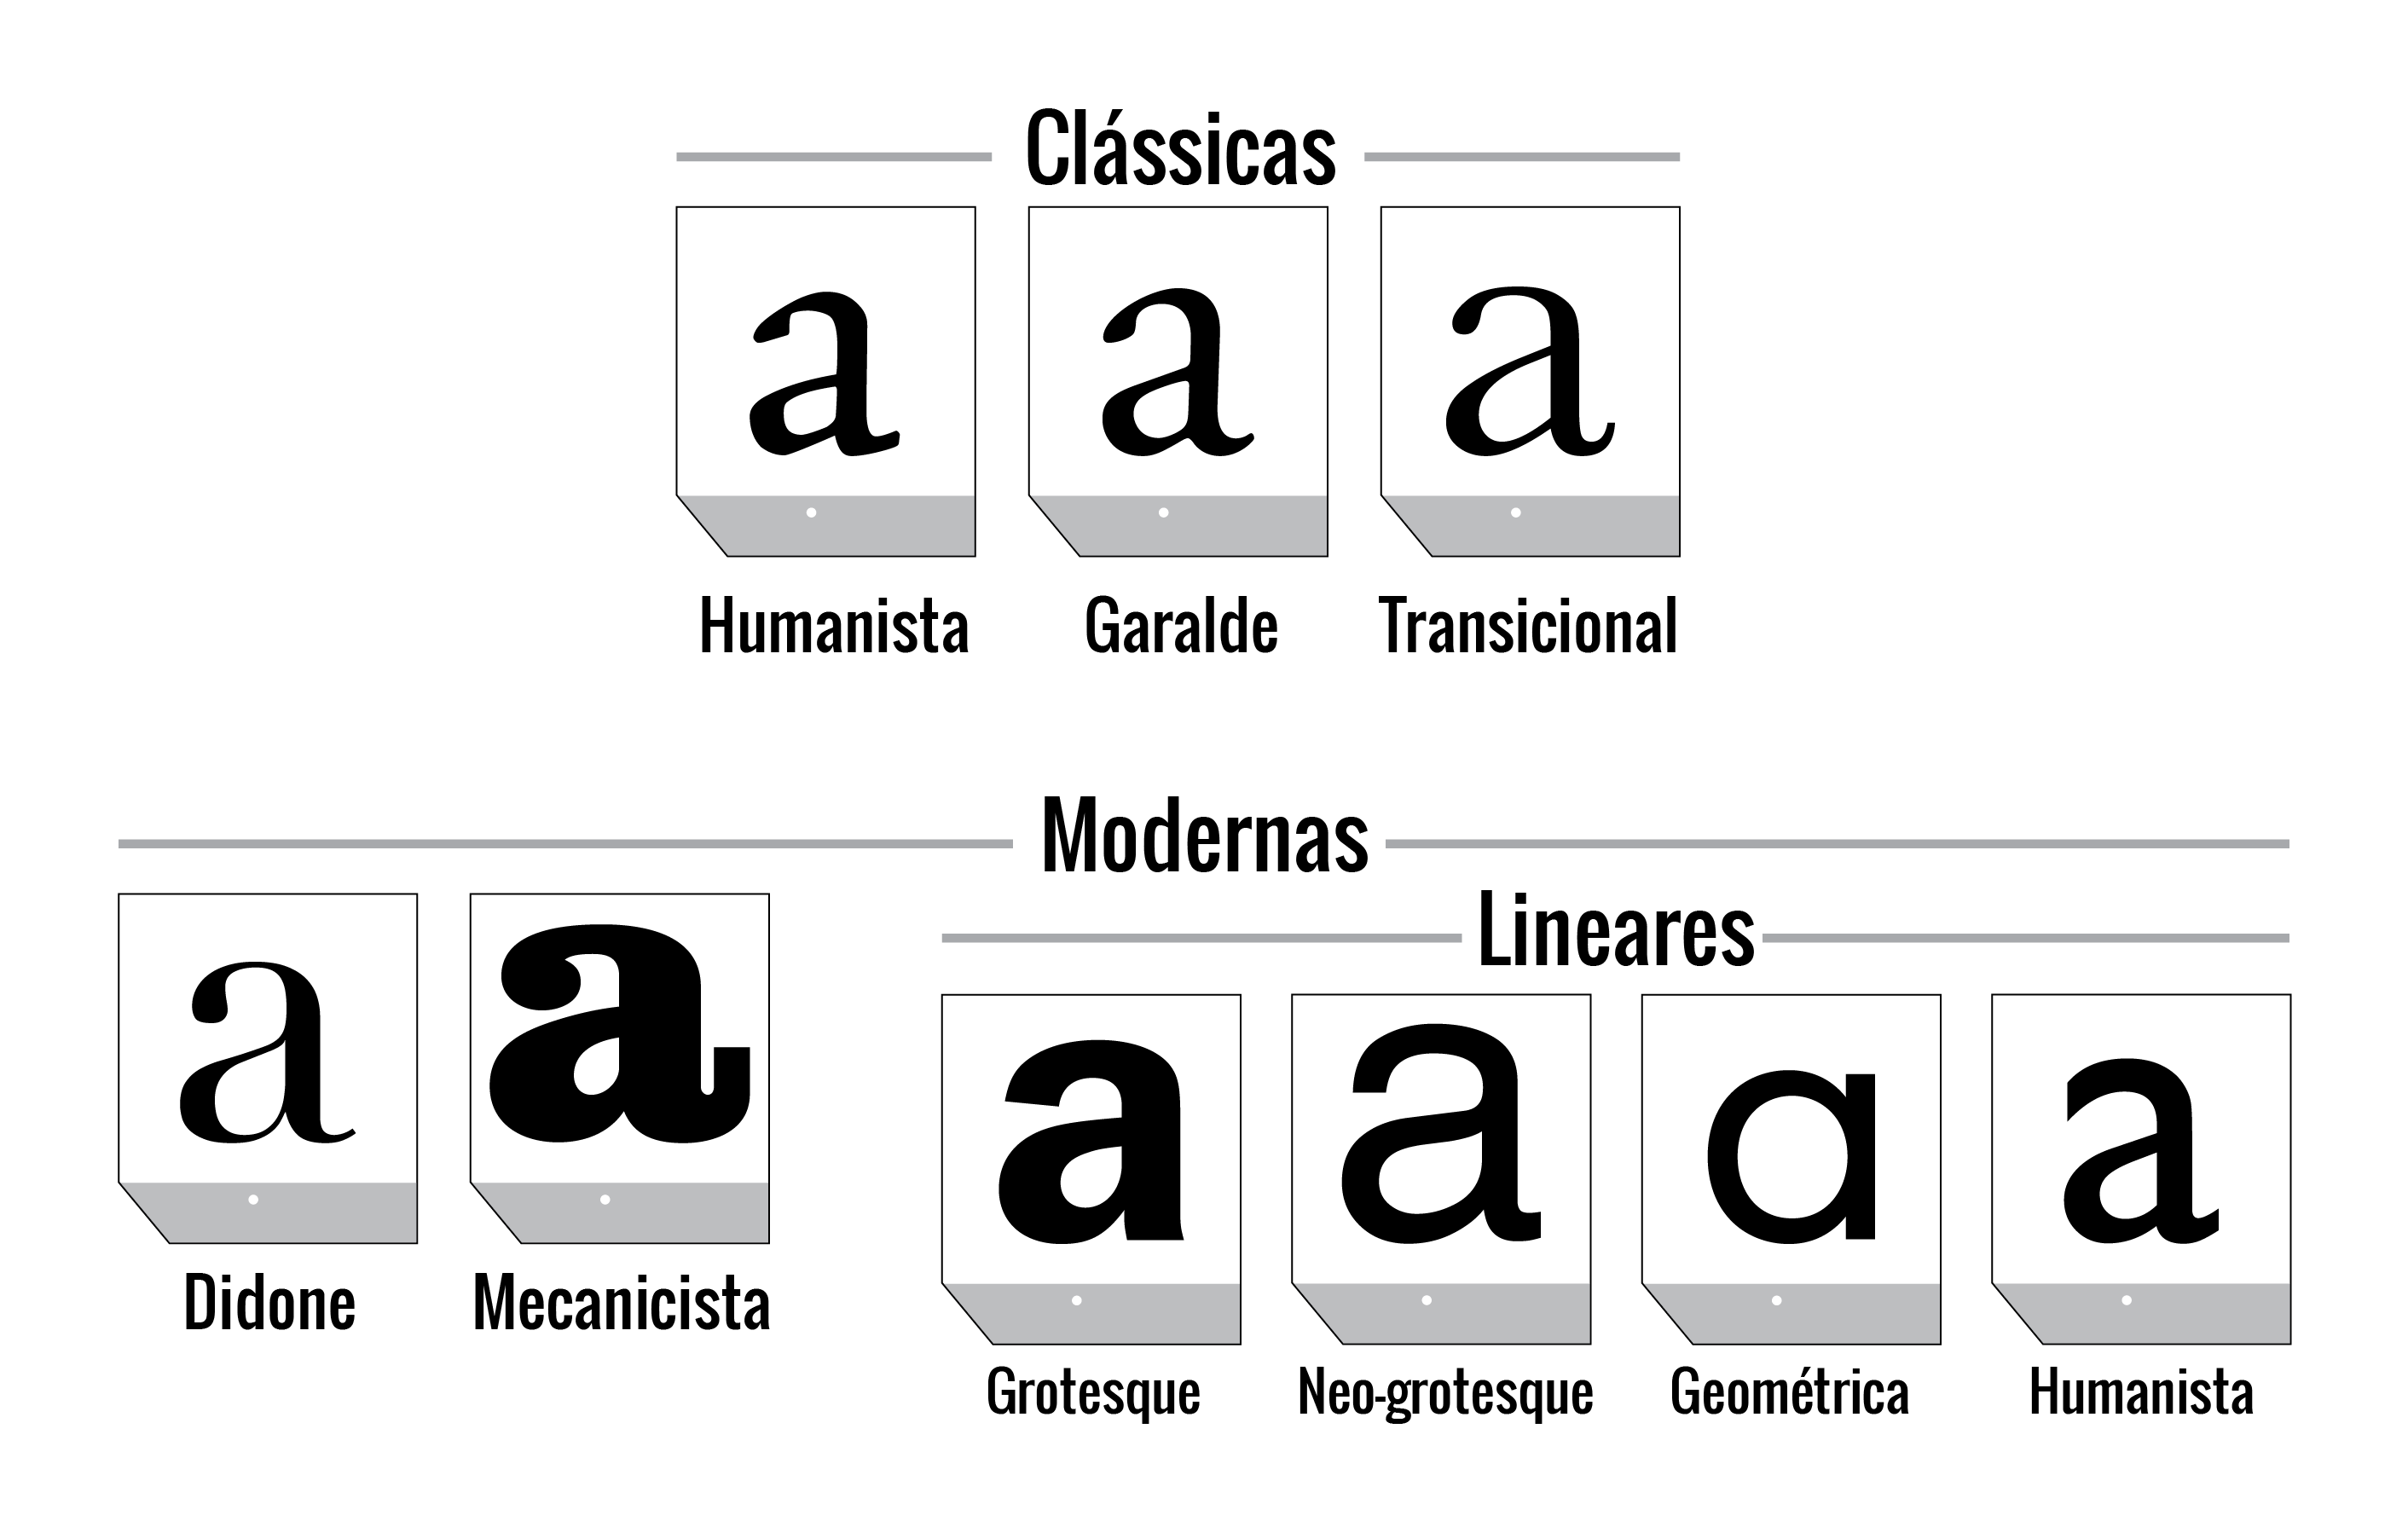
\includegraphics[width=0.7\linewidth]{figuras/categoriaProjeto.pdf}
  \caption{Categorias do sistema de classificação tipográfica Vox ATpyi que foram utilizadas no projeto \citeC{cruz2017}}
  \label{fig:categoriasProjeto}
\end{figure}

\section{Aplicações}

Como já retratado no Capítulo \ref{ch:intro}, um dos objetivos do projeto é mitigar a exclusão que o deficiente visual sofre em relação à várias áreas do conhecimento humano, dentre elas, a cultura e as artes. Sendo assim, pretende-se apresentar a tipografia por meio de uma tecnologia assistiva, que fornece explicações sobre as características e os conceitos, exemplificando por meio de aplicações reais das tipografias do projeto. Alguns exemplos práticos do uso das tipografias contidas no projeto são apresentados na Figura \ref{fig:marcas}. Observe que, dentre os exemplos, estão marcas de carros, equipamentos eletrônicos e roupas.


\begin{figure}[H]
 \centering
  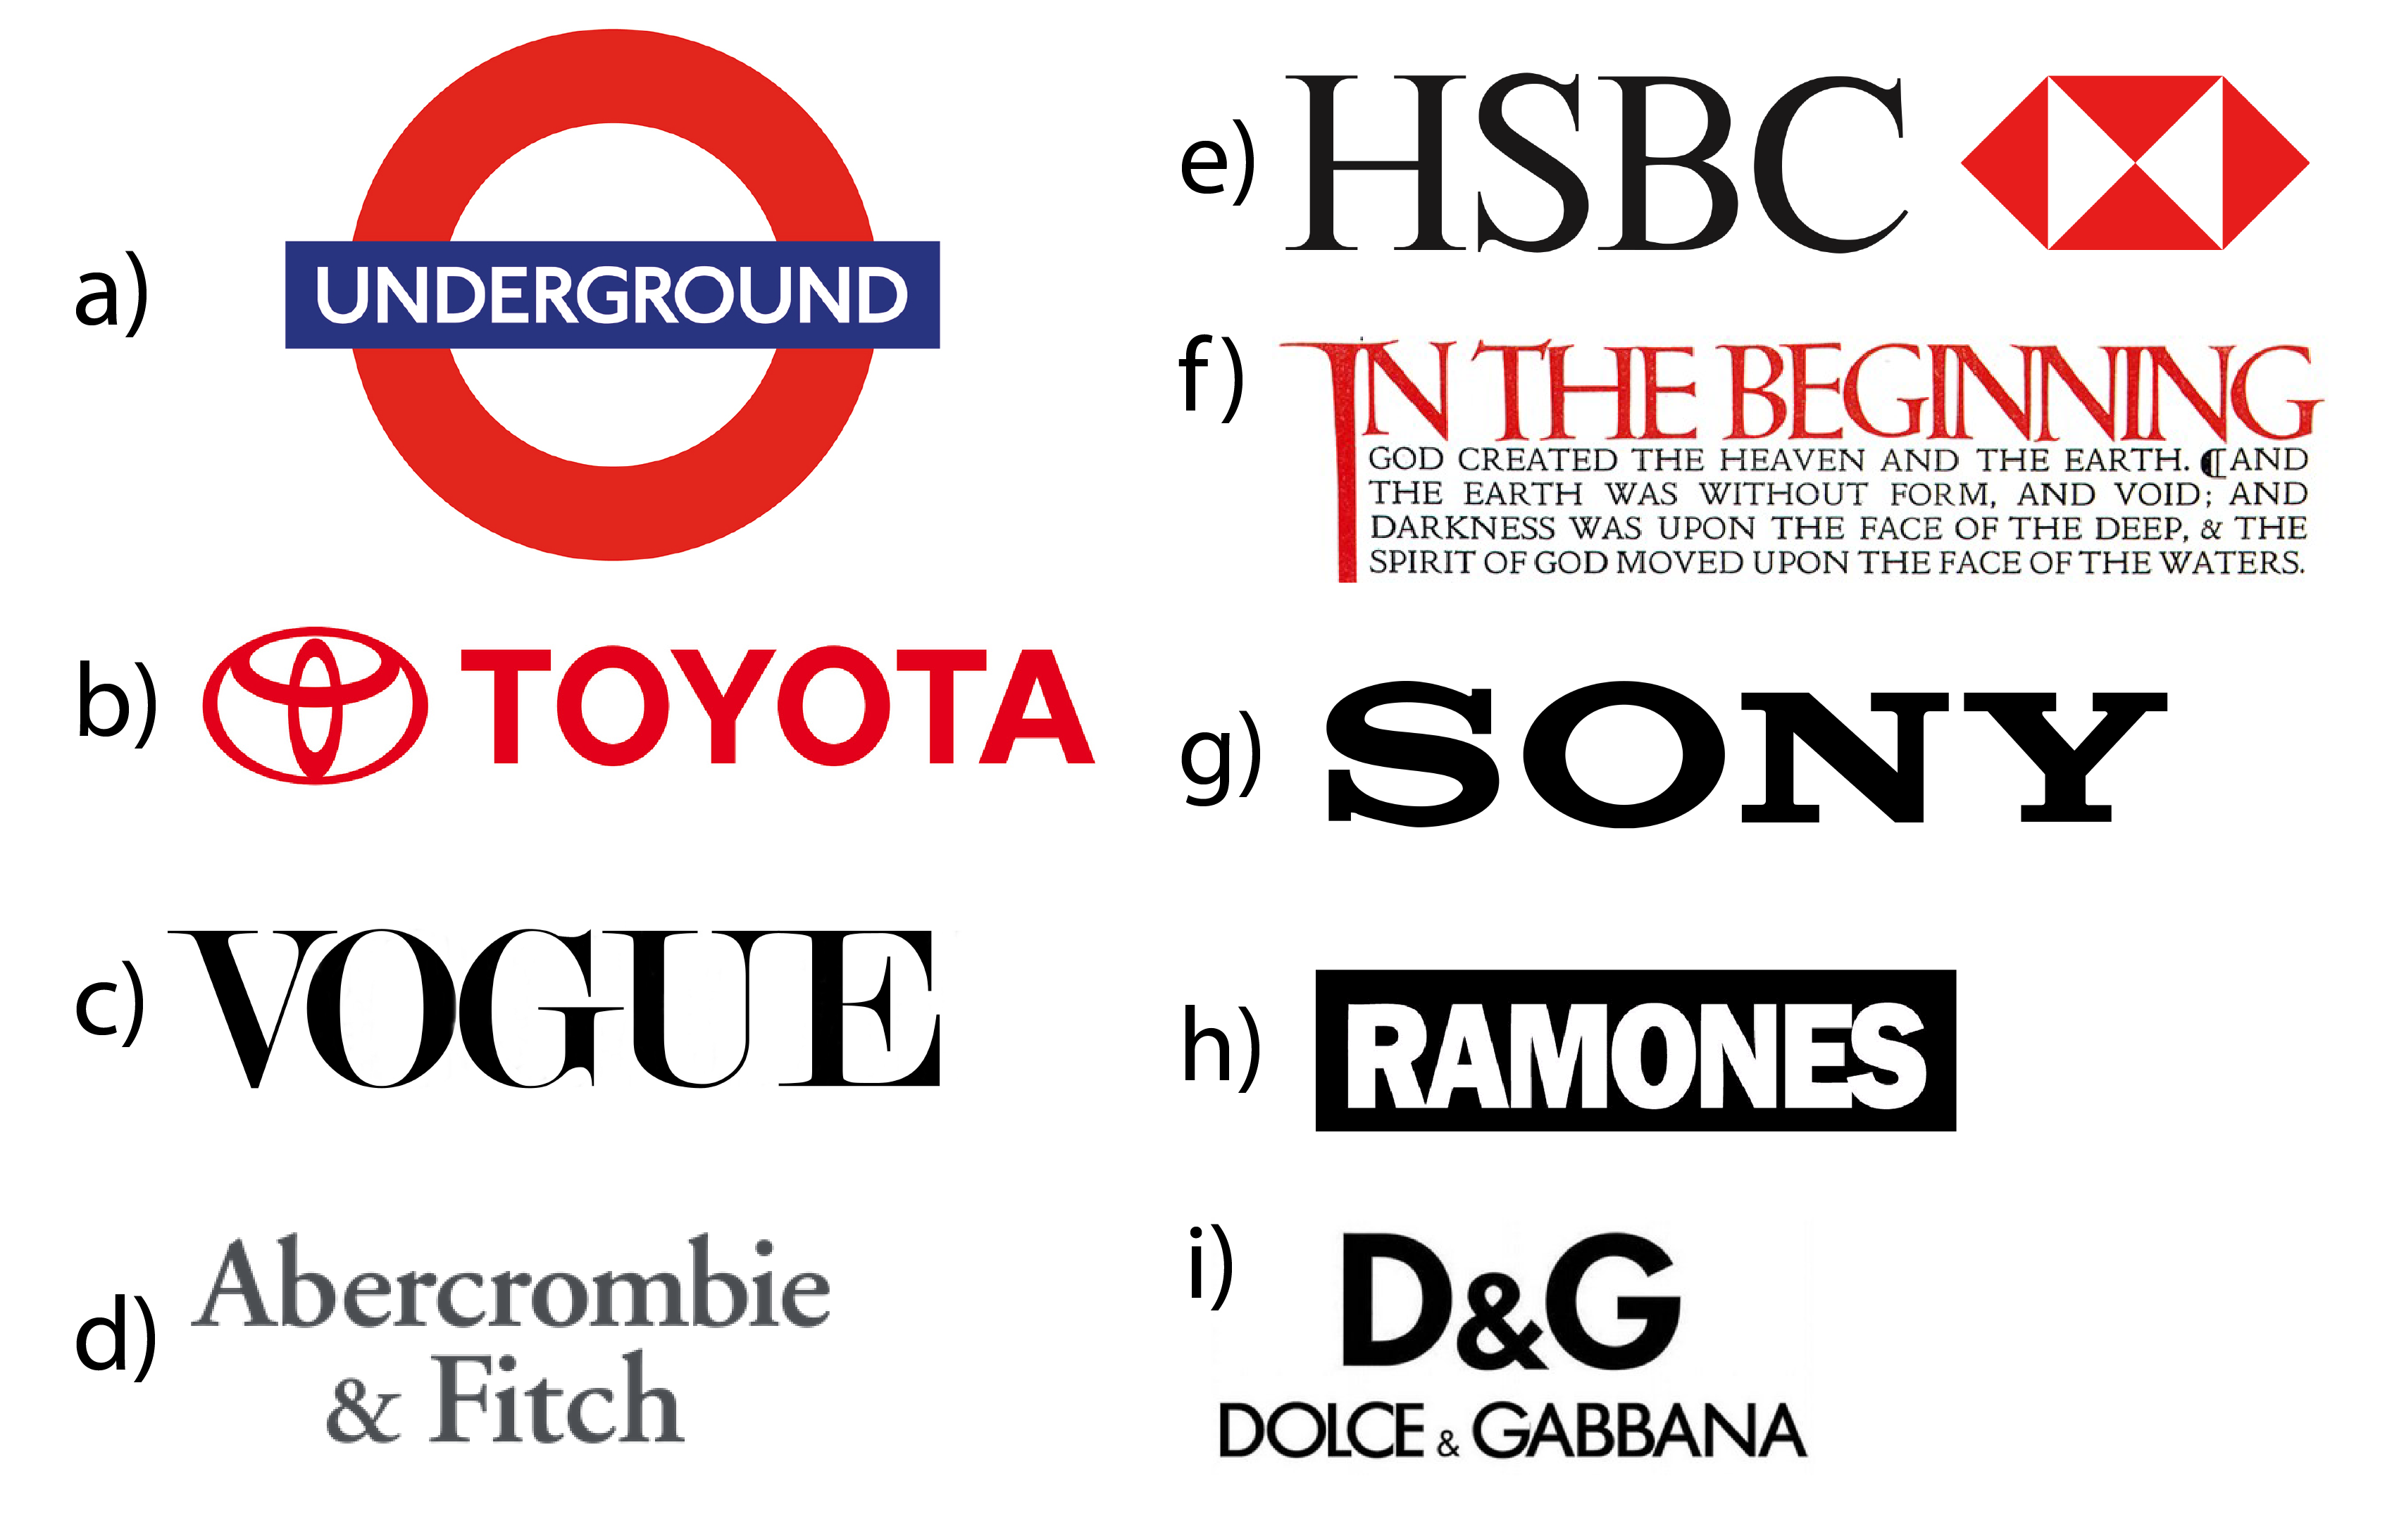
\includegraphics[width=0.7\linewidth]{figuras/logos.pdf}
  \caption{Exemplos de aplicação das tipografias presentes no projeto: a) Gill Sans, b) Helvetica, c) Didot, d) Garamond, e) Baskerville, f) Bíblia \textit{Dove Press} de 1902, g) Clarendon, h) Franklin Gothic, i) Futura.}
  \label{fig:marcas}
\end{figure}




